
\begin{frame}
\frametitle{MSNE in a Larger Game}
\begin{itemize}
	\item Suppose that we have this 3$\times$2 game:
\end{itemize}
\begin{table}[h]
\centering
\begin{tabular}{cr|c|c|}
	& \multicolumn{1}{c}{} & \multicolumn{2}{c}{Player 2}\\
	& \multicolumn{1}{c}{} & \multicolumn{1}{c}{X (r)}  & \multicolumn{1}{c}{Y (1 - r)} \\\cline{3-4}
	\multirow{3}*{Player 1}  & A (p) & 2, 1 & 0, 1 \\\cline{3-4}
	& B (q) & 1, 2 & 2, 0 \\\cline{3-4}
	& C (1 - p - q) & 0, 0 & 3, 2 \\\cline{3-4}
\end{tabular}
\end{table}
\begin{itemize}
	\item Player 1's mixed strategy uses probabilities p, q, and 1 - p - q, since they have three pure strategies.
\end{itemize}
\end{frame}

% - - - - - - - - - - - - - - - - - - - - - - - - - - - - - - - - - - - - - - -

\begin{frame}{Existence of Nash equilibria}
\frametitle{MSNE in a Larger Game}
\begin{itemize}
	\item Algebraically:
	\begin{itemize}
		\item $U_1(A) = 2r + 0 = 2r$.
		\item $U_1(B) = 1r + 2(1 - r) = 2 - r$.
		\item $U_1(C) = 0 + 3(1 - r) = 3 - 3r$.
	\end{itemize}
	\end{itemize}
\end{frame}

% - - - - - - - - - - - - - - - - - - - - - - - - - - - - - - - - - - - - - - -

\begin{frame}{Graph Player 1's expected utilities}
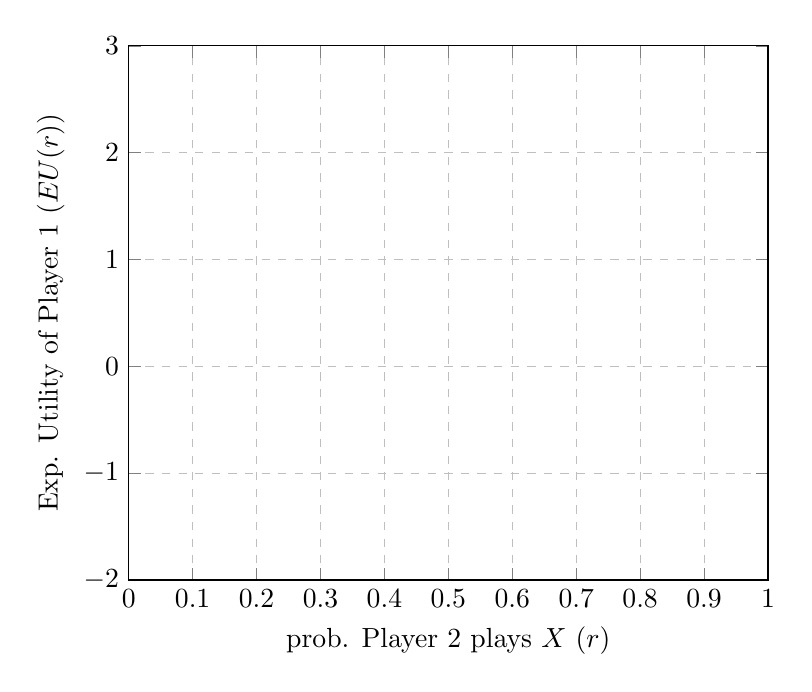
\begin{tikzpicture}
 
   \begin{axis}[
     width=0.8\textwidth,
     grid,
     xlabel={prob. Player 2 plays $X$ ($r$) },
     ylabel={Exp. Utility of Player 1 ($EU(r)$)},
     xmin=0, xmax=1.0,
     ymin=-2, ymax=3,
     xtick={0,.1,...,1.0},
     ytick={-2, -1, 0, 1, 2, 3},
     grid style=dashed,
     ]
 
     \addplot[draw=none] coordinates {(1,1)};
   \end{axis}
 \end{tikzpicture}
\end{frame}

% - - - - - - - - - - - - - - - - - - - - - - - - - - - - - - - - - - - - - - -

\begin{frame}{When will Player 1 mix?}
  \begin{itemize}
    \item What it would take to get Player 1 to mix different pairs of strategies:
	\begin{itemize}
		\item A and B: $2r = 2 - r \implies r = \frac{2}{3}$.
		\item A and C: $2r = 3 - 3r \implies r = \frac{3}{5}$.
		\item B and C: $2 - r = 3 - 3r \implies r = \frac{1}{2}$.
	\end{itemize}

    \item Note that there is no intersection between all three lines simultaneously

    \item This means that Player 1 will never mix between all three strategies
  \end{itemize}
\end{frame}

% - - - - - - - - - - - - - - - - - - - - - - - - - - - - - - - - - - - - - - -

\begin{frame}
\frametitle{MSNE in a Larger Game}
\begin{itemize}
	\item Let's check Player 2's expected payoffs next:
	\begin{itemize}
		\item $U_2(X) = 1p + 2q + 0$.
		\item $U_2(Y) = 1p + 0 + 2(1 - p - q)$.
	\end{itemize}
	\item So Player 2 will play a mixed strategy if
  $$p + 2q = p + 2(1 - p - q)$$ 
  $$\implies q = 1 - p - q$$.

  \begin{itemize}
    \item Recall that $q$ was the probability we put on Player 2 playing $B$,
    \item and $1-p-q$ was the probability they play $C$. 
  \end{itemize}

\end{itemize}
\end{frame}

% - - - - - - - - - - - - - - - - - - - - - - - - - - - - - - - - - - - - - - -

\begin{frame}{visualizing Player 2's Best Responses}
  \begin{center}
  \begin{tikzpicture}
    \draw (0,0) coordinate[label=below:$A$] (a) --
    (5,0) coordinate[label=below:$C$] (c) --
    (2.5, 4.3) coordinate[label=above:$B$] (b) -- cycle ;
  \end{tikzpicture}
  \end{center}
\end{frame}

% - - - - - - - - - - - - - - - - - - - - - - - - - - - - - - - - - - - - - - -

\begin{frame}{When will Player 2 mix?}
  \begin{itemize}
    \item We found they are indifferent between $X$ and $Y$ when 
    $$ q = 1 - p - d $$.

	  \item There are two ways that this can be true: 
    \begin{itemize}
      \item Either Player 1 plays B and C with equal probability
      (and we know from earlier that they would \textbf{only} be playing these two, not A),
      \item or Player 1 plays A only, and B and C not at all. 
    \end{itemize}
  \end{itemize}
\end{frame}

% - - - - - - - - - - - - - - - - - - - - - - - - - - - - - - - - - - - - - - -

\begin{frame}
\frametitle{MSNE in a Larger Game}
\underline{Case 1}: Player 1 only plays A:
\begin{itemize}
  \item this requires $2r \geq 2 - r$ and $2r \geq 3 - 3r$,
  \item which imply that $r \geq \frac{2}{3}$ and $r \geq \frac{3}{5}$.
  \item \textbf{MSNE 1:} \{(1, 0, 0), (r, 1 - r)\}, where $r \geq \frac{2}{3}$.
	\end{itemize}
\end{frame}

% - - - - - - - - - - - - - - - - - - - - - - - - - - - - - - - - - - - - - - -

\begin{frame}{MSNE in a Larger Game}
\underline{Case 2}: Player 1 plays $B$ and $C$ with equal probability 
  \begin{itemize}
   \item then Player 2 plays X and Y with equal (1/2) probability.
    \item \textbf{MSNE}: \{(0, 1/2, 1/2), (1/2, 1/2)\}
  \end{itemize} 
\end{frame}

% - - - - - - - - - - - - - - - - - - - - - - - - - - - - - - - - - - - - - - -

\begin{frame}{What about a 3x3 game?}
\begin{table}[h]
\centering
  \begin{tabular}{cr|c|c|c|}
	& \multicolumn{1}{c}{} & \multicolumn{3}{c}{Player 2}\\
    & \multicolumn{1}{c}{} & Rock ($r_2$) & Paper ($p_2$) & Scissors ($1-r_2-p_2$) \\\cline{3-5}
    \multirow{3}*{Player 1}  & Rock ($r_1$) & 0, 0 & -1, 1 & 1, -1 \\\cline{3-5}
    & Paper ($p_1$) & 1, -1 & 0,0 & -1, 1 \\\cline{3-5}
    & Scissors  & -1, 1 & 1, -1 & 0, 0 \\\cline{3-5}
\end{tabular}
\end{table}
\end{frame}

% - - - - - - - - - - - - - - - - - - - - - - - - - - - - - - - - - - - - - - -

\begin{frame}{What about a 3x3 game?}
  \begin{itemize}
    \item Rock, Paper, Scissors is a \textit{symmetric} game, so let's just pay attention to Player 1's utility 

    \item $EU_1(Rock | r_2, p_2) = $

    \item $EU_1(Paper | r_2, p_2) = $

    \item $EU_1(Scissors | r_2, p_2) = $
  \end{itemize}
  
\end{frame}

\begin{frame}{visualizing Player 1's Best Responses}
  \begin{center}
  \begin{tikzpicture}
    \draw (0,0) coordinate[label=below:$Rock$] (r) --
    (8,0) coordinate[label=below:$Paper$] (p) --
    (4, 7) coordinate[label=above:$Scissors$] (s) -- cycle ;
  \end{tikzpicture}
  \end{center}
\end{frame}

% - - - - - - - - - - - - - - - - - - - - - - - - - - - - - - - - - - - - - - -

\begin{frame}{Finding MSNE in 3x3 game}
  \begin{minipage}{0.45\textwidth}
  \begin{center}
  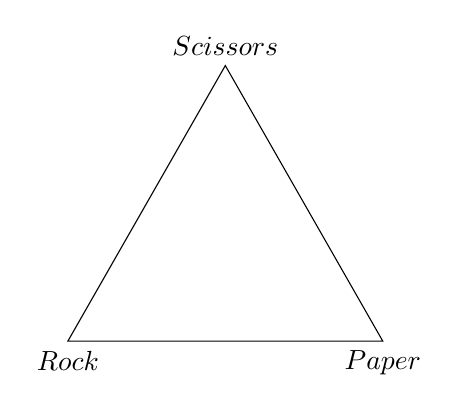
\begin{tikzpicture}
    \draw (0,0) coordinate[label=below:$Rock$] (r) --
    (4,0) coordinate[label=below:$Paper$] (p) --
    (2, 3.5) coordinate[label=above:$Scissors$] (s) -- cycle ;
  \end{tikzpicture}
  \end{center}
  \end{minipage} 
  \begin{minipage}{0.45\textwidth}
  \begin{center}
  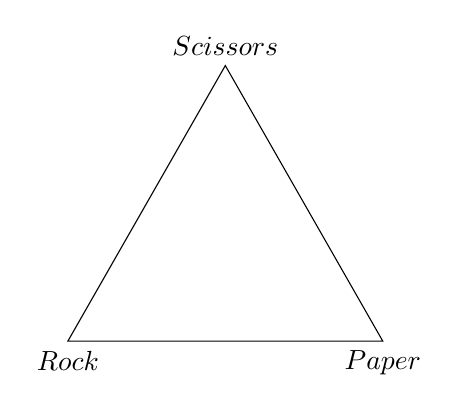
\begin{tikzpicture}
    \draw (0,0) coordinate[label=below:$Rock$] (r) --
    (4,0) coordinate[label=below:$Paper$] (p) --
    (2, 3.5) coordinate[label=above:$Scissors$] (s) -- cycle ;
  \end{tikzpicture}
  \end{center}
  \end{minipage} 
\end{frame}

% - - - - - - - - - - - - - - - - - - - - - - - - - - - - - - - - - - - - - - -

\begin{frame}{Finding MSNE in 3x3 game}
  So the results from our math confirm our intuition that the stable strategies in equilibrium are:
  \begin{itemize}
    \item Player 1 plays Rock with $r=1/3$, Paper with $p=1/3$, and Scissors with
    $1-p-r=1/3$
    \item Player 1 plays Rock with $r=1/3$, Paper with $p=1/3$, and Scissors with
    $1-p-r=1/3$
  \end{itemize}
\end{frame}

% - - - - - - - - - - - - - - - - - - - - - - - - - - - - - - - - - - - - - - -

\begin{frame}{Another 3x3 game}
 \begin{table}[h]
\centering
  \begin{tabular}{cr|c|c|c|}
	& \multicolumn{1}{c}{} & \multicolumn{3}{c}{Player 2}\\
    & \multicolumn{1}{c}{}            &  Left  & Center & Right  \\\cline{3-5}
    \multirow{3}*{Player 1}  & Top    &  2,  1 &  3,  0 &  3,  0 \\\cline{3-5}
                             & Middle &  3,  0 &  0,  1 &  3,  0 \\\cline{3-5}
                             & Bottom &  3,  0 &  3,  0 &  2,  1 \\\cline{3-5}
\end{tabular}
\end{table}
\end{frame}

% - - - - - - - - - - - - - - - - - - - - - - - - - - - - - - - - - - - - - - -

\begin{frame}{Solving for 3-strategy MSNE}
  \textbf{Step 1:} Define Mixed Strategies
  \begin{itemize}

    \item \underline{Player 1's mixed strategy:} 
    Let $\sigma_1 = (t, m, b)$  

    \item \underline{Player 2's mixed strategy:} 
    Let $\sigma_2 = (\ell, c, r)$  

  \end{itemize}
  
  Note that the lowercase letters represent the probabilities played
  on the uppercase pure strategies.
\end{frame}

% - - - - - - - - - - - - - - - - - - - - - - - - - - - - - - - - - - - - - - -

\begin{frame}{Solving for 3-strategy MSNE}
  \textbf{Step 2:} Solve for Expected Utilities

  \begin{multicols}{2}
  \begin{minipage}{.5\textwidth}
  \begin{itemize}
    
    \item \underline{Player 1:}
    \begin{itemize}

      \item $EU_1(T, \sigma_2) = $
      \vspace{8mm}

      \item $EU_1(M, \sigma_2) = $
      \vspace{8mm}

     \item $EU_1(B, \sigma_2) = $
      \vspace{8mm}
      
    \end{itemize}
  \end{itemize}
  \end{minipage}

  \begin{minipage}{.5\textwidth}
  \begin{itemize}
    
    \item \underline{Player 2:}
    \begin{itemize}

      \item $EU_2(L, \sigma_1) = $
      \vspace{8mm}
      \item $EU_2(C, \sigma_1) = $
      \vspace{8mm}
      \item $EU_2(R, \sigma_1) = $
      \vspace{8mm}
      
    \end{itemize}
  \end{itemize}
  \end{minipage}
  \end{multicols}

\end{frame}

% - - - - - - - - - - - - - - - - - - - - - - - - - - - - - - - - - - - - - - -

\begin{frame}{Solving for 3-strategy MSNE}
  \textbf{Step 3:} Find Indifference Conditions
  \begin{itemize}

    \item \underline{When will Player 1 mix between 2 pure strategies?} 
    \begin{itemize}
      \item When does $EU_1(Top, \sigma_2) = EU_1(Middle, \sigma_2)$:
      \vspace{14mm}
      \item When does $EU_1(Top, \sigma_2) = EU_1(Bottom, \sigma_2)$:
      \vspace{14mm}
      \item When does $EU_1(Middle, \sigma_2) = EU_1(Bottom, \sigma_2)$:
      \vspace{14mm}
      
    \end{itemize}
    
  \end{itemize}
  
\end{frame}

% - - - - - - - - - - - - - - - - - - - - - - - - - - - - - - - - - - - - - - -

\begin{frame}{Solving for 3-strategy MSNE}
  \textbf{Step 3:} Find Indifference Conditions
  \begin{itemize}

    \item \underline{When will Player 2 mix between 2 pure strategies?} 
    \begin{itemize}
      \item When does $EU_2(Left, \sigma_1) = EU_2(Center, \sigma_1)$:
      \vspace{14mm}
      \item When does $EU_2(Left, \sigma_1) = EU_2(Right, \sigma_1)$:
      \vspace{14mm}
      \item When does $EU_2(Center, \sigma_1) = EU_2(Right, \sigma_1)$:
      \vspace{14mm}
      
    \end{itemize}
    
  \end{itemize}
  
\end{frame}

% - - - - - - - - - - - - - - - - - - - - - - - - - - - - - - - - - - - - - - -

\begin{frame}{Solving for 3-strategy MSNE}
  \textbf{Step 4.a:} Graph Indifference Points on Number Lines for Player 1

  \vspace{60mm}
  
\end{frame}

% - - - - - - - - - - - - - - - - - - - - - - - - - - - - - - - - - - - - - - - 

\begin{frame}{Solving for 3-strategy MSNE}
  \textbf{Step 4.b:} Combine Number Lines into Player 1's BR Triangle
  \begin{center}
  \begin{tikzpicture}
    \draw (0,0) coordinate[label=below:Left] (r) --
    (6,0) coordinate[label=below:Right] (p) --
    (3, 5) coordinate[label=above:Center] (s) -- cycle ;
  \end{tikzpicture}
  \end{center}
\end{frame}

% - - - - - - - - - - - - - - - - - - - - - - - - - - - - - - - - - - - - - - - 

\begin{frame}{Solving for 3-strategy MSNE}
  \textbf{Step 4.c:} Graph Indifference Points on Number Lines for Player 2

  \vspace{60mm}
  
\end{frame}

% - - - - - - - - - - - - - - - - - - - - - - - - - - - - - - - - - - - - - - - 

\begin{frame}{Solving for 3-strategy MSNE}
  \textbf{Step 4.d:} Combine Number Lines into Player 2's BR Triangle
  \begin{center}
  \begin{tikzpicture}
    \draw (0,0) coordinate[label=below:Top] (r) --
    (6,0) coordinate[label=below:Bottom] (p) --
    (3, 5) coordinate[label=above:Middle] (s) -- cycle ;
  \end{tikzpicture}
  \end{center}
\end{frame}

% - - - - - - - - - - - - - - - - - - - - - - - - - - - - - - - - - - - - - - - 

\begin{frame}{Solving for 3-strategy MSNE}
  \textbf{Step 5:} Check Cases for possible Nash Equilibria:

  \vspace{60mm}
  
\end{frame}

% - - - - - - - - - - - - - - - - - - - - - - - - - - - - - - - - - - - - - - - 

